%%%%%%%%%%%%%%%%%%%%%%%%%%%%%%%%%%%%%%%%%%%%%%%%%%%%%%%%%%%%%%%%%%%%%%%%%
%  Zawartość: Główny plik dokumentacji projektowej GRAVIsim
%  Opracował: Adam Dłubak <adam.dlubak@gmail.com>
%  Data: Czerwiec 2017
%  Wersja: 1.0
%%%%%%%%%%%%%%%%%%%%%%%%%%%%%%%%%%%%%%%%%%%%%%%%%%%%%%%%%%%%%%%%%%%%%%%%%


\documentclass[a4paper,onecolumn,oneside,12pt]{memoir} 
\renewcommand{\normalsize}{\fontsize{12pt}{18pt}\selectfont}

\usepackage[utf8]{inputenc} % jeśli kodowanie edytowanych plików to UTF8
\usepackage[T1]{fontenc}
\usepackage[polish]{babel}
%\DisemulatePackage{setspace}
\usepackage{setspace}
\usepackage{tabularx}
\usepackage{color,calc}
\usepackage{soul} % pakiet z komendami do podkreślania tekstu
\usepackage{url}
\usepackage{framed}	
\usepackage[T1]{fontenc}% for \textbackslash inside \texttt
\usepackage{ebgaramond} % pakiet z czcionkami garamond, potrzebny tylko do strony tytułowej, musi wystąpić przed pakietem tgtermes

%% Aby uzyskać polskie literki w pdfie korzystam z pakietu czcionek tgterms. 
%% W pakiecie tym są zdefiniowane klony czcionek Times o kształtach: normalny, pogrubiony, italic, italic pogrubiony.
%% W pakiecie tym brakuje czcionki o kształcie: slanted (podobny do italic). 
%% Jeśli w dokumencie gdzieś zostanie zastosowana czcionka slanted (np. po użyciu komendy \textsl{}), to
%% latex dokona podstawienia na czcionkę standardową i zgłosi to w ostrzeżeniu (warningu).
%% Ponadto tgtermes to czcionka do tekstu. Wszelkie matematyczne wzory będą sformatowane domyślną czcionką do wzorów.
%% Jeśli wzory mają być sformatowane z wykorzystaniem innych czcionek, trzeba to jawnie zadeklarować.

%% Po zainstalowaniu pakietu tgtermes może będzie trzeba zauktualizować informacje 
%% o dostępnych fontach oraz mapy. Można to zrobić z konsoli (jako administrator)
%% initexmf --admin --update-fndb
%% initexmf --admin --mkmaps

\usepackage{tgtermes}   
\renewcommand*\ttdefault{txtt}

\usepackage{listings} % pakiet do prezentacji kodu. 

% Choć możliwe jest zastosowanie różnych pakietów formatujących tabele, zaleca się tego nie robić.
%\usepackage{longtable}
%\usepackage{ltxtable}
%\usepackage{tabulary}

%%%%%%%%%%%%%%%%%%%%%%%%%%%%%%%%%%%%%%%%%%%%%%%%%%%
%% Ustawienia odpowiedzialne za sposób łamania dokumentu
%% i ułożenie elementów pływających
%%%%%%%%%%%%%%%%%%%%%%%%%%%%%%%%%%%%%%%%%%%%%%%%%%%
%\hyphenpenalty=10000		% nie dziel wyrazów zbyt często
\clubpenalty=10000      	% kara za sierotki
\widowpenalty=10000  		% nie pozostawiaj wdów
\brokenpenalty=10000		% nie dziel wyrazów między stronami
\exhyphenpenalty=999999		% nie dziel słów z myślnikiem
\righthyphenmin=3			% dziel minimum 3 litery

\renewcommand{\topfraction}{0.95}
\renewcommand{\bottomfraction}{0.95}
\renewcommand{\textfraction}{0.05}
\renewcommand{\floatpagefraction}{0.35}

%%%%%%%%%%%%%%%%%%%%%%%%%%%%%%%%%%%%%%%%%%%%%%%%%%%
%%  Ustawienia rozmiarów: tekstu, nagłówka i stopki, marginesów
%%  dla dokumentów klasy memoir 
%%%%%%%%%%%%%%%%%%%%%%%%%%%%%%%%%%%%%%%%%%%%%%%%%%%
\setlength{\headsep}{10pt} 
\setlength{\headheight}{13.6pt} % wartość baselineskip dla czcionki 11pt tj. \small wynosi 13.6pt
\setlength{\footskip}{\headsep+\headheight}
\setlength{\uppermargin}{\headheight+\headsep+1cm}
\setlength{\textheight}{\paperheight-\uppermargin-\footskip-1.5cm}
\setlength{\textwidth}{\paperwidth-5cm}
\setlength{\spinemargin}{2.5cm}
\setlength{\foremargin}{2.5cm}
\setlength{\marginparsep}{2mm}
\setlength{\marginparwidth}{2.3mm}
%\settrimmedsize{297mm}{210mm}{*}
%\settrims{0mm}{0mm}	
\checkandfixthelayout[fixed] % konieczne, aby się dobrze wszystko poustawiało
%%%%%%%%%%%%%%%%%%%%%%%%%%%%%%%%%%%%%%%%%%%%%%%%
%%  Ustawienia odległości linii, wcięć, odstępów
%%%%%%%%%%%%%%%%%%%%%%%%%%%%%%%%%%%%%%%%%%%%%%%%
\linespread{1}
%\linespread{1.241}
\setlength{\parindent}{14.5pt}
%\setbeforesecskip{10pt plus 0.5ex}%{-3.5ex \@plus -1ex \@minus -.2ex}
%\setaftersecskip{10pt plus 0.5ex}%\onelineskip}
%\setbeforesubsecskip{8pt plus 0.5ex}%{-3.5ex \@plus -1ex \@minus -.2ex}
%\setaftersubsecskip{8pt plus 0.5ex}%\onelineskip}
%\setlength\floatsep{6pt plus 2pt minus 2pt} 
%\setlength\intextsep{12pt plus 2pt minus 2pt} 
%\setlength\textfloatsep{12pt plus 2pt minus 2pt} 

%%%%%%%%%%%%%%%%%%%%%%%%%%%%%%%%%%%%%%%%%%%%%%%%%%%
%%  Pakiety i komendy zastosowane tylko do zamieszczenia informacji o użytych komendach i fontach
%%  Normalnie nie są potrzebne, można je zamarkować podczas redakcji pracy
%%%%%%%%%%%%%%%%%%%%%%%%%%%%%%%%%%%%%%%%%%%%%%%%%%%
\usepackage{memlays}     % extra layout diagrams, zastosowane w szblonie do 'debuggowania', używa pakietu layouts
%\usepackage{layouts}
\usepackage{printlen} % pakiet do wyświetlania wartości zdefiniowanych długości, stosowany do 'debuggowania'
\uselengthunit{pt}
\makeatletter
\newcommand{\showFontSize}{\f@size pt} % makro wypisujące wielkość bieżącej czcionki
\makeatother
% do pokazania ramek można byłoby użyć:
%\usepackage{showframe} 



%%%%%%%%%%%%%%%%%%%%%%%%%%%%%%%%%%%%%%%%%%%%%%%%%%%
%%  Formatowanie list wyliczeniowych, wypunktowań i własnych otoczeń
%%%%%%%%%%%%%%%%%%%%%%%%%%%%%%%%%%%%%%%%%%%%%%%%%%%

% Domyślnie wypunktowania mają zadeklatorowane znaki, które nie występują w tgtermes
% Aby latex nie podstawiał w ich miejsca znaków z czcionki standardowej można zrobić podstawienie:
%    \DeclareTextCommandDefault{\textbullet}{\ensuremath{\bullet}}
%    \DeclareTextCommandDefault{\textasteriskcentered}{\ensuremath{\ast}}
%    \DeclareTextCommandDefault{\textperiodcentered}{\ensuremath{\cdot}}
% Jednak jeszcze lepszym pomysłem jest zdefiniowanie otoczeń z wykorzystaniem enumitem
\usepackage{enumitem} % pakiet pozwalający zarządzać formatowaniem list wyliczeniowych
\setlist{noitemsep,topsep=4pt,parsep=0pt,partopsep=4pt,leftmargin=*} % zadeklarowane parametry pozwalają uzyskać 'zwartą' postać wypunktowania bądź wyliczenia
\setenumerate{labelindent=0pt,itemindent=0pt,leftmargin=!,label=\arabic*.} % można zmienić \arabic na \alph, jeśli wyliczenia mają być z literkami
\setlistdepth{4} % definiujemy głębokość zagnieżdżenia list wyliczeniowych do 4 poziomów
\setlist[itemize,1]{label=$\bullet$}  % definiujemy, jaki symbol ma być użyty w wyliczeniu na danym poziomie
\setlist[itemize,2]{label=\normalfont\bfseries\textendash}
\setlist[itemize,3]{label=$\ast$}
\setlist[itemize,4]{label=$\cdot$}
\renewlist{itemize}{itemize}{4}

%%%http://tex.stackexchange.com/questions/29322/how-to-make-enumerate-items-align-at-left-margin
%\renewenvironment{enumerate}
%{
%\begin{list}{\arabic{enumi}.}
%{
%\usecounter{enumi}
%%\setlength{\itemindent}{0pt}
%%\setlength{\leftmargin}{1.8em}%{2zw} % 
%%\setlength{\rightmargin}{0zw} %
%%\setlength{\labelsep}{1zw} %
%%\setlength{\labelwidth}{3zw} % 
%\setlength{\topsep}{6pt}%
%\setlength{\partopsep}{0pt}%
%\setlength{\parskip}{0pt}%
%\setlength{\parsep}{0em} % 
%\setlength{\itemsep}{0em} % 
%%\setlength{\listparindent}{1zw} % 
%}
%}{
%\end{list}
%}

\makeatletter
\renewenvironment{quote}{
	\begin{list}{}
	{
	\setlength{\leftmargin}{1em}
	\setlength{\topsep}{0pt}%
	\setlength{\partopsep}{0pt}%
	\setlength{\parskip}{0pt}%
	\setlength{\parsep}{0pt}%
	\setlength{\itemsep}{0pt}
	}
	}{
	\end{list}}
\makeatother

%%%%%%%%%%%%%%%%%%%%%%%%%%%%%%%%%%%%%%%%%
%%  Pakiet do generowania indeksu (ważne, aby wstawić przed hyperref)
%%%%%%%%%%%%%%%%%%%%%%%%%%%%%%%%%%%%%%%%%
\DisemulatePackage{imakeidx}
\usepackage[makeindex,noautomatic]{imakeidx} % tutaj mówimy, żeby indeks nie generował się automatycznie, 

%\usepackage[noautomatic]{imakeidx} 
\makeindex

\makeatletter
%%%\renewenvironment{theindex}
							 %%%{\vskip 10pt\@makeschapterhead{\indexname}\vskip -3pt%
								%%%\@mkboth{\MakeUppercase\indexname}%
												%%%{\MakeUppercase\indexname}%
								%%%\vspace{-3.2mm}\parindent\z@%
								%%%\renewcommand\subitem{\par\hangindent 16\p@ \hspace*{0\p@}}%%
								%%%\phantomsection%
								%%%\begin{multicols}{2}
								%%%%\thispagestyle{plain}
								%%%\parindent\z@                
								%%%%\parskip\z@ \@plus .3\p@\relax
								%%%\let\item\@idxitem}
							 %%%{\end{multicols}\clearpage}
%%%
\makeatother


\usepackage{ifpdf}
%\newif\ifpdf \ifx\pdfoutput\undefined
%\pdffalse % we are not running PDFLaTeX
%\else
%\pdfoutput=1 % we are running PDFLaTeX
%\pdftrue \fi
\ifpdf
 \usepackage[pdftex,bookmarks,breaklinks,unicode]{hyperref}
 \usepackage[pdftex]{graphicx}
 \DeclareGraphicsExtensions{.pdf,.jpg,.mps,.png}
\pdfcompresslevel=9
\pdfoutput=1
\makeatletter
\AtBeginDocument{
  \hypersetup{  
    allbordercolors=0 0 0,
    pdfborderstyle={/S/U/W 0},
	pdfinfo={
    Title = {\@title},
    Author = {\@author},
    Subject={},
    Keywords={słowa kluczowe},
  }}
}
\makeatother
\else
\usepackage{graphicx}
\DeclareGraphicsExtensions{.eps,.ps,.jpg,.mps,.png}
\fi
\sloppy


%\graphicspath{{rys01/}{rys02/}}


%%%%%%%%%%%%%%%%%%%%%%%%%%%%%%%%%%%%%%%%%
% Metadane dla pdfa


%\ifpdf
%\pdfinfo{
   %/Author (Nicola Talbot)
   %/Title  (Creating a PDF document using PDFLaTeX)
   %/CreationDate (D:20040502195600)
   %/ModDate (D:\pdfdate)
   %/Subject (PDFLaTeX)
   %/Keywords (PDF;LaTeX)
%}
%\fi

% Deklaracja głębokościu numeracji
\setcounter{secnumdepth}{2}
\setcounter{tocdepth}{2}
\setsecnumdepth{subsection} % activating subsubsec numbering in doc


% Kropki po numerach sekcji
\makeatletter
\def\@seccntformat#1{\csname the#1\endcsname.\quad}
\def\numberline#1{\hb@xt@\@tempdima{#1\if&#1&\else.\fi\hfil}}
\makeatother

\renewcommand{\chapternumberline}[1]{#1.\quad}
\renewcommand{\cftchapterdotsep}{\cftdotsep}

%\definecolor{niceblue}{rgb}{.168,.234,.671}

% Czcionka do podpisów tabel i rysunków
\captionnamefont{\small}
\captiontitlefont{\small}
% makro pozwalające zmienić sposób wypisywania rozdziału
%\def\printchaptertitle##1{\fonttitle \space \thechapter.\space ##1} 

%\usepackage{ltcaption}
% The ltcaption package supports \CaptionLabelFont & \CaptionTextFont introduced by the NTG document classes
%\renewcommand\CaptionLabelFont{\small}
%\renewcommand\CaptionTextFont{\small}

% Przedefiniowanie etykiet w podpisach tabel i rysunków
%\AtBeginDocument{% 
        \addto\captionspolish{% 
        \renewcommand{\tablename}{Tab.}% 
}%} 

%\AtBeginDocument{% 
%        \addto\captionspolish{% 
%        \renewcommand{\chaptername}{Rozdział}% 
%}} 

%\AtBeginDocument{% 
        \addto\captionspolish{% 
        \renewcommand{\figurename}{Rys.}% 
}%}


%\AtBeginDocument{% 
        \addto\captionspolish{% 
        \renewcommand{\bibname}{Literatura}% 
}%}

%\AtBeginDocument{% 
        \addto\captionspolish{% 
        \renewcommand{\listfigurename}{Spis rysunków}% 
}%}

%\AtBeginDocument{% 
        \addto\captionspolish{% 
        \renewcommand{\listtablename}{Spis tabel}% 
}%}

%\AtBeginDocument{% 
        \addto\captionspolish

%%%%%%%%%%%%%%%%%%%%%%%%%%%%%%%%%%%%%%%%%%%%%%%%%%%%%%%%%%%%%%%%%%                  
%% Definicje stopek i nagłówków
%%%%%%%%%%%%%%%%%%%%%%%%%%%%%%%%%%%%%%%%%%%%%%%%%%%%%%%%%%%%%%%%%%                  
\addtopsmarks{headings}{%
\nouppercaseheads % added at the beginning
}{%
\createmark{chapter}{both}{shownumber}{}{. \space}
%\createmark{chapter}{left}{shownumber}{}{. \space}
\createmark{section}{right}{shownumber}{}{. \space}
}%use the new settings

\makeatletter
\copypagestyle{outer}{headings}
\makeoddhead{outer}{}{}{\small\itshape\rightmark}
\makeevenhead{outer}{\small\itshape\leftmark}{}{}
\makeoddfoot{outer}{\small\@author:~\@titleShort}{}{\small\thepage}
\makeevenfoot{outer}{\small\thepage}{}{\small\@author:~\@title}
\makeheadrule{outer}{\linewidth}{\normalrulethickness}
\makefootrule{outer}{\linewidth}{\normalrulethickness}{2pt}
\makeatother

% fix plain
\copypagestyle{plain}{headings} % overwrite plain with outer
\makeoddhead{plain}{}{}{} % remove right header
\makeevenhead{plain}{}{}{} % remove left header
\makeevenfoot{plain}{}{}{}
\makeoddfoot{plain}{}{}{}

\copypagestyle{empty}{headings} % overwrite plain with outer
\makeoddhead{empty}{}{}{} % remove right header
\makeevenhead{empty}{}{}{} % remove left header
\makeevenfoot{empty}{}{}{}
\makeoddfoot{empty}{}{}{}


%%%%%%%%%%%%%%%%%%%%%%%%%%%%%%%%%%%%%%%
%% Definicja strony tytułowej 
%%%%%%%%%%%%%%%%%%%%%%%%%%%%%%%%%%%%%%%
\makeatletter
%Uczelnia
\newcommand\uczelnia[1]{\renewcommand\@uczelnia{#1}}
\newcommand\@uczelnia{}
%Wydział
\newcommand\wydzial[1]{\renewcommand\@wydzial{#1}}
\newcommand\@wydzial{}
%Kierunek
\newcommand\kierunek[1]{\renewcommand\@kierunek{#1}}
\newcommand\@kierunek{}
%Specjalność
\newcommand\specjalnosc[1]{\renewcommand\@specjalnosc{#1}}
\newcommand\@specjalnosc{}
%Kurs
\newcommand\kurs[1]{\renewcommand\@kurs{#1}}
\newcommand\@kurs{}

%Tytuł krótki
\newcommand\titleShort[1]{\renewcommand\@titleShort{#1}}
\newcommand\@titleShort{}
%Prowadzacy
\newcommand\prowadzacy[1]{\renewcommand\@prowadzacy{#1}}
\newcommand\@prowadzacy{}

\def\maketitle{%
  \pagestyle{empty}%
%%\garamond 
	\fontfamily{\ebgaramond@family}\selectfont % na stronie tytułowej czcionka garamond
%%%%%%%%%%%%%%%%%%%%%%%%%%%%%%%%%%%%%	
%% Poniżej, w otoczniu picture, wstawiono tytuł i autora. 
%% Tytuł (z autorem) musi znaleźć się w obszarze 
%% odpowiadającym okienku 110mmx75mm, którego lewy górny róg 
%% jest w położeniu 77mm od lewej i 111mm od górnej  krawędzi strony 
%% (tak wynika z wycięcia na okładce). 
%% Poniższy kod musi być użyty dokładnie w miejscu gdzie jest.
%% Jeśli tytuł nie mieści się w okienku, to należy tak pozmieniać 
%% parametry użytych komend, aby ten przydługi tytuł jednak 
%% upakować go do okienka.
%%
%% Sama okładka (kolorowa strona z wycięciem, do pobrania z dydaktyki) 
%% powinna być przycięta o 3mm od każdej z krawędzi.
%% Te 3mm pewnie zostawiono na ewentualne spady czy też specjalną oprawę.
%%%%%%%%%%%%%%%%%%%%%%%%%%%%%%%%%%%%%	
\newlength{\tmpfboxrule}
\setlength{\tmpfboxrule}{\fboxrule}
\setlength{\fboxsep}{2mm}
\setlength{\fboxrule}{0mm} 
%\setlength{\fboxrule}{0.1mm} %% jeśli chcemy zobaczyć ramkę
\setlength{\unitlength}{1mm}
\begin{picture}(0,0)
\put(-70,-214.5){\fbox{
\parbox[c][11mm][c]{124mm}{\centering %\lineskip=34pt 


		\fontsize{16pt}{18pt}\selectfont AUTORZY:\\[3mm]
		\fontsize{14pt}{16pt}\selectfont Adam Dłubak\\[1mm]
		\fontsize{14pt}{16pt}\selectfont Jakub Błaszczyk\\[10mm]		
		}
%\fontsize{15pt}{18pt}\selectfont AUTORZY:\\[2mm]
%\fontsize{14pt}{16pt}\selectfont \@author\\[2mm]
%\fontsize{14pt}{16pt}\selectfont Jakub Błaszczyk}
}
}
\end{picture}
\setlength{\fboxrule}{\tmpfboxrule} 
%%%%%%%%%%%%%%%%%%%%%%%%%%%%%%%%%%%%%
%% Reszta strony z nazwą uczelni, wydziału, kierunkiem, specjalnością
%% promotorem, oceną pracy, miastem i rokiem
	{\centering%\vspace{-1cm}
		{\fontsize{22pt}{24pt}\selectfont \@uczelnia}\\[0.4cm]
		{\fontsize{22pt}{24pt}\selectfont \@wydzial}\\[0.5cm]
		  \hrule %\vspace*{0.7cm}
	}
{\flushleft\fontsize{14pt}{16pt}\selectfont%
\begin{tabular}{ll}
KIERUNEK: & \@kierunek\\
SPECJALNOŚĆ: & \@specjalnosc\\
KURS: & \@kurs\\
\end{tabular}\\[5.3cm]
}
{\centering
{\fontsize{32pt}{36pt}\selectfont \@title}\\[0.5cm]
{\fontsize{26pt}{30pt}\selectfont Dokumentacja projektowa}\\[2.5cm]
}
\vfill
\begin{tabularx}{\linewidth}{p{10cm}l}
		&{\fontsize{16pt}{18pt}\selectfont PROWADZĄCY:}\\[2mm] %UWAGA: tutaj jest miejsce na nazwisko promotora pracy
		&{\fontsize{14pt}{16pt}\selectfont \@prowadzacy}\\[10mm]

	\end{tabularx}
\vspace{2cm}
\hrule\vspace*{0.3cm}


{\centering
{\fontsize{16pt}{18pt}\selectfont \@date}\\[0cm]
}
%\ungaramond
\normalfont

\newpage
}
\makeatother
%%%%%%%%%%%%%%%%%%%%%%%%%%%%%%%%%%%%%%%%%

%\AtBeginDocument{\addtocontents{toc}{\protect\thispagestyle{empty}}}




%%%%%%%%%%%%%%%%%%%%%%%%%%%%%%%%%%%%%%%%%
%%  Metadane dokumentu 
%%%%%%%%%%%%%%%%%%%%%%%%%%%%%%%%%%%%%%%%%
\title{GRAVISIM}
\titleShort{Grawitacyjna symulacja N-ciał}
\author{Adam Dłubak, Jakub Błaszczyk}
\uczelnia{POLITECHNIKA WROCŁAWSKA}
\wydzial{WYDZIAŁ ELEKTRONIKI}
\kierunek{INFORMATYKA}
\specjalnosc{INŻYNIERIA INTERNETOWA}
\kurs{APLIKACJE INTERNETOWE I ROZPROSZONE}
\prowadzacy{Dr inż. Marek Woda}
\date{WROCŁAW, 2017}

% Ustawienie odstępu od góry w nienumerowanych rozdziałach oraz wykazach:
% Spis treści, Spis tabel, Spis rysunków, Indeks rzeczowy

%\newlength{\linespace}
%\setlength{\linespace}{-\beforechapskip-\topskip+\headheight+\topsep}
%\makechapterstyle{noNumbered}{%
%\renewcommand\chapterheadstart{\vspace*{\linespace}}
%}

%% powyższa komenda załatwia to, co robią komendy poniższe dla spisów
%\renewcommand*{\tocheadstart}{\vspace*{\linespace}}
%\renewcommand*{\lotheadstart}{\vspace*{\linespace}}
%\renewcommand*{\lofheadstart}{\vspace*{\linespace}}

%%%%%%%%%%%%%%%%%%%%%%%%%%%%%%%%%%%%%%%%%
%                  Początek dokumentu 
%%%%%%%%%%%%%%%%%%%%%%%%%%%%%%%%%%%%%%%%%
%\includeonly{skroty,rozdzial01} % jeśli chcemy kompilować tylko fragmenty, to można tu je wpisać

\begin{document}
% Tutaj można przełączyć odstęp między liniami
%\SingleSpacing
%\OnehalfSpacing
%\DoubleSpacing

%\settypeoutlayoutunit{cm} % do debugowania
%\typeoutstandardlayout    % wypisuje na stdout informacje o ustawieniach
\maketitle

\chapterstyle{noNumbered}
\pagestyle{outer}
\mbox{}\pdfbookmark[0]{Spis treści}{spisTresci.1}
\tableofcontents* 


\chapter{Wprowadzenie} \label{rozdz.Wprowadzenie} 
{\em \quad \quad \textbf{GRAVIsim} to narzędzie umożliwiające przeprowadzanie astrofizycznej symulacji grawitacyjnej N-ciał zaimplementowane w systemie rozproszonym. Interfejsem symulacji jest aplikacja internetowa pozwalająca autoryzowanym członkom instytutu badawczego na zlecanie oraz analizowanie (interpretowanie) zadań badawczych.
}

\section{Pomysł, motywacja, stan rynku}
\quad \quad Pomysł stworzenia GRAVIsim zrodził się w głowach autorów poprzez ich zamiłowanie do astrofizyki. Operowanie na systemach rozproszonych doskonale wpasowuje się w tematykę przetwarzania dużej ilości informacji, potrzebnej do przeprowadzenia symulacji zderzeń kosmicznych. \\
\\
Z racji, iż na ogólnodostępnym rynku brak jest aplikacji wykonującej podobne zadania, autorzy GRAVIsim mieli silną motywację do stworzenia narzędzia, które mogłoby zobrazować zjawisko zderzeń astrofizycznych występujących w kosmosie, jednak niedostrzegalnych dla człowieka. \\
\\
Dzięki stworzeniu środowiska pozwalającego zarządzać symulacjami można lepiej poznać oraz zobrazować siły oddziaływania grawitacyjnego w makroskali. Wyniki takich badań mogą być wykorzystywane zarówno przez naukowców jak i w celach popularnonaukowych. Dzięki możliwości zobrazowania, w formie graficznej animacji, wyników przeprowadzonych badań narzędzie to może promować takie dziedziny nauki jak fizyka i astronomia wśród dzieci, młodzieży, ale również i osób dorosłych.

\section{Zarys projektu}
\quad \quad GRAVIsim to z jednej strony narzędzie pozwalające zarządzać klastrem obliczeniowym złożonym z dowolnej liczby komputerów klasy PC w celu wykonywania konkretnych obliczeń na sieci rozproszonej, z drugiej - jest to prosta i przyjazna w użytkowaniu aplikacja internetowa. Zalogowany użytkownik może dzięki niej wykorzystać potencjał obliczeniowy klastra do symulowania zderzeń grawitacyjnych dowolnej liczby obiektów kosmicznych (np. planet, gwiazd, gromad, galaktyk). Aplikacja obsługuje cały proces takiego zadania zaczynając od utworzenia danych wejściowych, poprzez zlecenie pomiarów, jego monitorowanie, kończąc aż na analizie danych końcowych i jej graficznej wizualizacji.



\section{Przeznaczenie projektu}
\quad \quad Celem projektu jest stworzenie symulacji grawitacyjnej N-ciał wraz z interfejsem webowym pozwalającym na zlecanie badań dla różnych scen/obiektów i graficzna interpretacja otrzymanych wyników.\\
Projekt przeznaczony jest do celów naukowo-badawczych, obrazujący podstawową mechanikę oddziaływać grawitacyjnych. Skala i wartości obiektów symulacji (odległość, masa, siły) są rzeczywistym przekształceniem odpowiadających wartości świata rzeczywistego, co gwarantuje abstrakcyjnym obiektom symulacji faktyczną nośność informacji względem odpowiadających obiektom rzeczywistym.

\chapter{Zakres projektu}
{\emph{\quad \quad W pierwszej fazie projektu (jeszcze przed oficjalnym Kick-Off) został ustalony cel projektu, który w ramach kursu chcieliśmy osiągnąć, a także funkcjonalności, które aplikacja GRAVIsim powinna posiadać. Funkcjonalności te zostały podzielone na podstawowe oraz rozszerzone, czyli takie które nie są krytyczne dla założonego funkcjonowania systemu jednak ich zaimplementowanie jest dodatkową wartością dla systemu i będzie dużym udogodnieniem (lub rozszerzeniem możliwości) dla osób z niego korzystających.}


\section{Cel projektu}

\quad \quad Zbudowanie aplikacji internetowej, która poprzez interfejs użytkownika umożliwi obsługę zadań wykonywanych na systemie rozproszonym. 
Użytkowanie aplikacji możliwe jest poprzez dostęp do hermetycznego systemu, do którego użytkownik może dostać się jedynie poprzez poprawne jego zarejestrowanie w bazie przez administratora, a następnie zalogowanie do serwisu. 
Użytkownik systemu GRAVIsim po poprawnym zalogowaniu może wykonać następujące funkcjonalności:
\begin{itemize}
\item Generować dane wejściowe symulacji
\item Zlecać zadania z wcześniej wygenerowanego pliku
\item Zarządzać zadaniami – parametry takie jak: tytuł, opis, ilość iteracji, priorytet, status zadania
\item Obserwować postęp prowadzonej symulacji
\item Analizować wynik symulacji

\end{itemize}

\section{Funkcjonalności podstawowe}

\begin{itemize}\bfseries
\item Symulacja grawitacyjna N-ciał oparta na systemie rozproszonym
\end{itemize}
\begin{itemize}
\item[] Zaimplementowanie algorytmu dokładnego (zupełnego) operującego na systemie rozproszonym, który wykonuje symulacje grawitacyjne N-ciał. 
\end{itemize}
\pagebreak

\vspace*{1mm}
\begin{itemize}\bfseries
\item Interfejs webowy pozwalający na zlecenie oraz zarządzanie badaniami
\end{itemize}
\begin{itemize}
\item[] Stworzenie prostej, nowoczesnej i przyjaznej dla użytkownika aplikacji internetowej opartej o freamworki AngularJS oraz front-endowy Bootstrap. Serwis ma być intuicyjny oraz zapewniać dostęp do wszystkich możliwości jakie oferuje GRAVIsim. Użytkownik koniecznie musi mieć możliwość:

\begin{itemize}[leftmargin=+8mm]
\item Zlecać badania.
\item Konfigurować parametry oraz opis zadania.
\item Zarządzać statusem zadania (anulować, wstrzymywać, ustawiać w kolejce zadań).
\item Jako rezultat pomiarów otrzymać wizualizację wyników w formie poklatkowej animacji.
\end{itemize}

\end{itemize}

\begin{itemize}\bfseries
\item System uwierzytelniania użytkownika

\end{itemize}

\begin{itemize}
\item[] Powinien zostać zaprojektowany system uwierzytelniania użytkowników w aplikacji wraz z zaimplementowane następujące funkcjonalności:


\begin{itemize}[leftmargin=+8mm]
\item Rejestracja nowego użytkownika.
\item Logowanie w systemie.
\item Zarządzanie innymi użytkownikami poprzez konto administratora.
\item Automatyczne wygaszanie sesji w przypadku określonego czasu braku działań na koncie użytkownika.
\end{itemize}

\end{itemize}


\begin{itemize}\bfseries
\item Możliwość wprowadzenia danych wejściowych z poziomu aplikacji webowej
\end{itemize}
\begin{itemize}
\item[] Aplikacja powinna być wyposażona w formularz umożliwiający generowanie zadania z poziomu interfejsu oraz jego parametryzowanie poprzez:
\begin{itemize}
\item Wgrywanie pliku wejściowego z danymi.
\item Nazywanie i opisywanie zadania.
\item Ustawianie ilości iteracji.
\item Wybieranie priorytetu wykonywalności.
\end{itemize}
\end{itemize}

\begin{itemize}\bfseries
\item Graficzna interpretacja wyników
\end{itemize}
\begin{itemize}
\item[] Możliwość wizualnej interpretacji wyników wykonanego badania z poziomu szczegółowego widoku zadania w aplikacji. Okno animacji ma mieć możliwość:
\begin{itemize}
\item Wstrzymywania oraz ponowego uruchamiania animacji.
\item Ustawiania szybkości wyświetlanej animacji (\textit{FPS - Frame per second}).
\item Uruchamiania animacji w trybie pełnoekranowym.
\item Pobierania danych generujących animację (wynikowych badania).
\end{itemize}
\end{itemize}

\pagebreak
\vspace*{1mm}
\section{Funkcjonalności rozszerzone}


\begin{itemize}\bfseries
\item Historia badań
\end{itemize}
\begin{itemize}
\item[] Możliwość podglądu archiwalnych i obecnych zadań z pełną dostępnością informacji (parametry, logi, rezultaty) dla danego użytkownika oraz analogicznie dla wszystkich użytkowników jedynie z konta administratora.
\end{itemize}

\begin{itemize}\bfseries
\item Monitorowanie postępu prowadzonego badania
\end{itemize}
\begin{itemize}
\item[] Użytkownik ma mieć możliwość monitorowania postępu wykonywanego zadania w czasie rzeczywistym z poziomu aplikacji. Interfejs ma posiadać dane dotyczące stopnia wykonanego zadania (pasek postępu) wraz ze wszystkimi dodatkowymi informacjami w postaci logów systemowych.
\end{itemize}


\begin{itemize}\bfseries
\item Generator danych wejściowych
\end{itemize}
\begin{itemize}
\item[] Generator w formie graficznego narzędzia w przyjazny i intuicyjny dla użytkownika sposób ma generować dane wejściowe dla systemu badań grawitacyjnych. Generator ma umożliwiać:
\begin{itemize}
\item Tworzenie dwóch rodzajów próbek: pojedynczych punktów lub chmury punktów.
\item Dla pojedynczej próbki wybór koloru oraz masy.
\item Dla chmury próbek dodatkowo: rozmiar chmury oraz ilość pojedynczych próbek w chmurze.

\end{itemize}
\end{itemize}

\section{Wymagania technologiczne}

	Aplikacja kliencka powinna zostać zbudowana w oparciu o technologię \textbf{AngularJS}, w formie aplikacji typu \textit{One-Site-Page} w języku \textit{Javascript}. Obsługa danych w aplikacji ma być zapewniona przez framework \textbf{Django}, napisany w \textit{Python}. W celu zapewnienia aplikacji estetycznego wyglądu zastosowany zostanie framework \textbf{Boostrap} wraz z \textit{CSS3} oraz \textit{HTML5}. Do wspomagania autoryzacji będą używane \textbf{tokeny JWT}. Moduł aplikacji wykonujący obliczenia rozproszone będzie wykonany przy użyciu \textbf{Apache Spark}, natomiast komunikacja pomiędzy aplikacją, a dokładniej \textbf{Django Web API} oraz modułem obliczającym będzie opierać się o dedykowany moduł \textbf{Job Scheduler'a} oraz \textbf{Loggera} (do przesyłania informacji o stanie badań) napisanych w języku \textit{Python} oraz \textit{Javascript}.



\chapter{Charakterystyka projektu}
\section{Cykl życia aplikacji}
\quad \quad Każde zadanie przetwarzane jest przez wszystkie 4 podsystemy aplikacji. Moduł serwerowy
odpowiada za przetwarzanie takich zapytań jak tworzenie czy modyfikacja zleceń.
Moduł Spark Schedulera zarządza oczekującymi zleceniami przetwarzając ich stan
oraz przekazując do klastra. Moduł socketów pozwala na monitorowanie stanu zlecenia
w czasie rzeczywistym. Ponad to, szcegółowo informuje o wszystkich ewentualnych błędach
nieżależnie od źródła ich wystąpienia. Zewnętrzny moduł Spark odpowiada za przetwarzanie
otrzymanych zadań i generowanie symulacji.

Jako wynik pracy podsystemów jest gotowa symulacja w postaci pliku `JSON` wizualizowana
w wartwie prezentacji aplikacji klienckiej.

Pełen cykl życia zadania przedstawia poniższy diagram:

\begin{figure}[h]
	\centering
	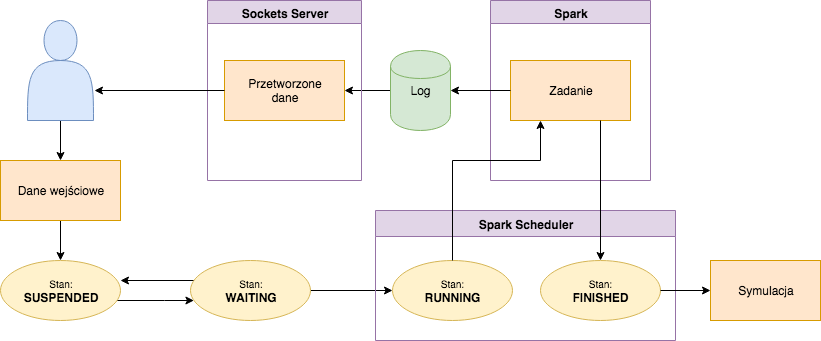
\includegraphics[width=1\linewidth]{lifecycle}
	\caption{Schemat modułów aplikacji GRAVIsim}
	\label{fig:stronaTytulowa}
\end{figure}

\section{Technologia}
\quad \quad Aplikacja podzielona została na kilka logicznych modułów, z których każdy pełni odrębną
rolę w całym cyklu życia. Można wyróżnić 4 podsystemy:
\begin{itemize}
\item Serwer Django - Aplikacja
\item Spark - Klaster
\item Spark Scheduler - Zarządzanie
\item Sockets server - Logger
\end{itemize}

\subsection{Moduł aplikacji (Django)}
\quad \quad Główny moduł aplikacji. Jego główną rolą jest przetwarzanie zapytań użytkowników,
serwowanie statycznych zasobów oraz zarządzanie całym stanem aplikacji.\\
\\
Serwer podzielony jest na 2 logiczne warstwy: serwerową oraz API. Pierwsza warstwa
pełni interfejs pomiędzy warstwą prezentacji (frontend) a cała logiką systemu.
Druga warstwa jest znacznie bardziej rozbudowana. Oparta na frameworku `Django REST
framework` zajmuje się przetwarzaniem oraz interpretacją zapytań pozwalając na
komunikację - odczyt bądź bezpieczny zapis danych - z bazą danych.\\
\\
Warstwa API jest głównym mechanizmem generowania zleceń badawczych. Zaimplementowane
mechanizmy serializacji dbają, aby użytkownik mógł być w stanie edytować tylko
wybrane pola przy określonych warunkach - eliminuje to ryzyko utraty spójności
danych.\\

\subsection{Moduł klastra (Apache Spark)}
\quad \quad 
\subsection{Moduł zarządzający (Spark-Scheduler)}
\quad \quad To główny moduł zarządzający wykonywanymi zadaniami. Podobnie jak serwer socketów
uruchamiany jest jako komenda głównego serwera. Jego główną ideą jest
przekazywanie oczekujących zadań zgodnie z ustaloną kolejnością priorytetów
do obliczeń w klastrze. Moduł odpowiedzialny jest zachowanie spójności zadań
(klaster równocześnie może obsłużyć tylko 1 zadanie) oraz ciągłość pracy
(po zakończeniu 1 zadania lub w stanie bezczyności, klaster autmatycznie otrzymuje
nowe zadanie).\\
\\
Zasada działania spark schedulera oparta jest na cyklicznym odpytywaniu bazy danych
w poszukiwaniu zadań oczekujących na dostępność klastra. Gdy w systemie znajdują się
takie zadania, moduł szereguje je zgodnie z ustaloną kolejką priorytetów (im wyższy
priorytet - tym szybciej zadanie zostanie obsłużone) oraz w przypadku równoznacznych
priorytetów - zgodnie z czasem oczekiwania (eliminacja zjawiska zagłodzenia).
Zadanie znajdujące się na początku kolejki jest blokowane poprzez zmianę stanu
na `RUNNING` oraz przekazane do klastra.\\
\\
Przekazanie zadania do obliczenia w klastrze odbywa się poprzez wywołanie komendy
`spark-submit` z odpowiednimi parametrami, przy użyciu funkcji Popen. Idea tego
rozwiązania pozwala na przekierowanie całego wyjścia komendy - zarówno zwykłych
komunikatów jak i błędów systemowych czy własnych infomarcji jak stan czy postęp
zadania - do określonego pliku zewnętrzengo służącego jako log zadania. Tak przekazane
zadanie może być asynchronicznie śledzone przez inne moduły oraz użytkoników końcowych.\\
\\
Po zakończeniu komendy - zarówno pozytywnego jak i w przypadku wystąpienia dowolnego
błędu - zadanie jest finalizowane poprzez ustawienie stanu na `FINISHED`. Rezultat
zadania przekazany jest automatycznie w logu zadania oraz w przypadku sukcesu -
plik symulacyjny jest zapisany na dysku serwera z ustaloną kowencją nazewnictwa
gwarantującą unikalność oraz dostępność.\\

\subsection{Moduł asynchroniczny (Socket-Server)}
\quad \quad Asynchroniczny moduł uruchamiany jako komenda głownego serwera. Pozwala on na
komunikację aplikacji klienckiej z serwerem za pośrednictwem otwartego na oddzielnym
porcie gniazda. Jego główna ideą jest umożliwienie asynchronicznego śledzenia
stanu i postępu zleconych badań oraz ewentualnych komunikatów błędów i ostrzeżeń.\\
\\
Główna zasada działania modułu opiera się cyklicznym odczycie zadanego pliku z logiem
zadania i przekazywaniu przetworzonej informacji do socketa. Bardzo ważnym aspektem
było zapewnienie nieblokującego przetwarzania - w przeciwnym wypadku serwer byłby
w stanie równocześnie obsłużyć tylko i wyłącznie 1 użytkownika.\\
\\
Zapytanie jest przetwarzane wg. poniższego schematu:
\begin{enumerate}
\item Utworzenie połączenia i określenie identyfikatora monitorowanego zadania
\item Sprawdzenie czy plik z logiem zadanie istnieje na serwerze: jeśli nie istnieje
to wysłanie komunikatu, że zadanie się jeszcze nie rozpoczęło, następnie nieblokujące
oczekiwanie przez 1000ms i ponownie krok 2
\item Ustalenie znacznika na początek pliku
\item Odczyt do bufora wszystkich linii od znacznika do końca pliku
\item Ustalenie znacznika na końcu pliku
\item Wysłanie do gniazda komunikatu z buforem linii
\item Nieblokujące oczekiwanie przez 500ms i powrót do kroku 4
\end{enumerate}

Połączenia po stronie serwera zamykane są automatycznie po zamknięciu ich w aplikacji
klienckiej.\\

\chapter{Implementacja}
\section{Aplikacja}
%podział na api, SPA na frontendzie, autoryzacja itp.
\section{Logger}
\section{Zarządzanie zadaniami}


\chapter{Instalacja i uruchomienie aplikacji}
{\emph{\quad \quad W celu uruchomienia aplikacji GRAVIsim ze wszystkimi jej funkcjonalnością, konieczna jest instalacja dodatkowych zależności, z których główną jest \textit{Apache Spark} zajmujący się obsługą klastra obliczeniowego.}
\section{Proces instalacji}
\definecolor{light-gray}{RGB}{226,226,226}
\sethlcolor{light-gray}
W pierwszej kolejności należy pobrać i zainstalować następujące oprogramowanie:


\begin{enumerate}

\item {
\textbf{Java SE Development Kit (SDK) w wersji 8 lub nowszej} - \underline{\href{http://www.oracle.com/technetwork/java/javase/downloads/jdk8-downloads-2133151.html}{Link do pobrania}}  \\
Aby zweryfikować poprawność instalacji, należy otworzyć konsolę (\texttt{\hl{cmd}}), wpisać \texttt{\hl{java}} i kliknąć \textit{Enter}. Jeśli pojawi się wiadomość: \\
 \centerline{\texttt{\hl{Java is not recognized as an internal or external command.}}}
lub podobna, należy:

\vspace{2mm}
\begin{quote}
\item \textbf{Windows:} skonfigurować zmienne środowiskowe: 	\texttt{\hl{JAVA{\char`_}HOME}} (podając ścieżkę do miejsca zainstalowania \textit{Java JDK}) oraz \texttt{\hl{PATH}} jako \texttt{\hl{\%JAVA{\char`_}HOME\%\textbackslash bin}} 
\end{quote}
\vspace{2mm}

\begin{enumerate}
\item Przejdź do Control \texttt{\hl{Panel\textbackslash System and Security\textbackslash System }}
\item Wybierz \texttt{\hl{Advance System Settings}} 
\item Wybierz \texttt{\hl{Environment Variables}}
\item W polu \texttt{\hl{user variables}} dodaj  nową zmienną środowiskową np. \texttt{\hl{SCALA{\char`_}HOME}} podając jako wartość ścieżkę do miejsca zainstalowania \textit{Scali}.
\item W polu \texttt{\hl{user variables}} edytuj zmienną \texttt{\hl{PATH}} dodając nowy klucz np. \texttt{\hl{\%SCALA{\char`_}HOME\%\textbackslash bin}}


\end{enumerate}

\vspace{2mm}
\begin{quote}
\item \textbf{Linux:} dodać ścieżkę z plikiem wykonywalnym do \texttt{\hl{PATH}}
\end{quote}
\vspace{2mm}


}

\item {
\textbf{Scala} - \underline{\href{http://www.scala-lang.org/download/}{Link do pobrania}}  \\
Gdy Scala zostanie zainstalowana, należy ustawić zmienne środowiskowe \texttt{\hl{SCALA{\char`_}HOME}} do folderu, gdzie zainstalowano \textit{Scalę} i \texttt{\hl{PATH}} jako \texttt{\hl{\%SCALA{\char`_}HOME\%\textbackslash bin}}.
}
\\
\item {
\textbf{Python w wersji 3.5} - \underline{\href{https://www.python.org/downloads/windows/}{Link do pobrania}}  
}
\\
\item {
\textbf{SBT} - \underline{\href{http://www.scala-sbt.org/download.html}{Link do pobrania}}  \\
Gdy \textit{SBT} zostanie zainstalowane, należy ustawić zmienną środowiskową  \texttt{\hl{SBT{\char`_}HOME}} jako ścieżkę do miejsca, gdzie zainstalowano \textit{SBT}.
}
\\
\item {
\textbf{WinUtils} - Tylko Windows - \underline{\href{http://public-repo-1.hortonworks.com/hdp-win-alpha/winutils.exe}{Link do pobrania}}  \\
Dopóki nie ma zainstalowanego lokalnego \textit{Hadoop’a} na Windows konieczne jest pobranie \texttt{\hl{winutils.exe}} i umieszczenia go w folderze \texttt{\hl{Hadoop/bin/}}, który należy uprzednio utworzyć w dowolnej lokalizacji na dysku, a następnie ustawić zmienną środowiskową :

\centerline{\texttt{\hl{HADOOP{\char`_}HOME = Lokalizacja{\char`_}utworzonego{\char`_}folderu{\char`_}Hadoop}}}
}

\vspace{6mm}
\item {
\textbf{Apache Spark z Hadoop 2.7} - \underline{\href{http://spark.apache.org/downloads.html}{Link do pobrania}}  \\
Należy wybrać najnowszą wersję oraz \textit{package type} jako \textit{Pre-built for Apache Hadoop 2.7 and later}. Gdy \textit{Spark} zostanie zainstalowany, należy ustawić zmienne środowiskowe: \texttt{\hl{SPARK{\char`_}HOME}} jako ścieżkę do miejsca, gdzie zainstalowano \textit{Spark’a} oraz dodać ścieżkę \texttt{\hl{\%SPARK{\char`_}HOME\%\textbackslash bin}} do \texttt{\hl{PATH}}.
}

\vspace{6mm}
\item {
\textbf{SSHFS} - \underline{\href{https://www.digitalocean.com/community/tutorials/how-to-use-sshfs-to-mount-remote-file-systems-over-ssh}{Link do instrukcji instalacji}} \\
Pozwala na podmontowanie poprzez \textit{ssh} lokalnie folderu z innej maszyny.
Jest to niezbędne przy klastrach składających się z więcej niż 1 maszyny.
}
\end{enumerate}
\vspace{6mm}
Po zakończonej instalacji można zweryfikować stan klastra wpisując komendę
{\texttt{\hl{Spark-shell}}} w konsoli systemowej. \textit{Apache Spark} powinien przejść proces instalacji i wyświetlić
charakterystyczny napis \textit{Spark}. Wówczas instalacja została zakończona pomyślnie.

\begin{figure}[h]
	\centering
	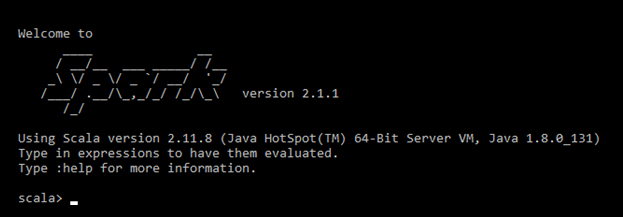
\includegraphics[width=1\linewidth]{spark-installed}
	\caption{Komunikat informujący o poprawnie zakończonej instalacji Apache Spark}
	\label{fig:stronaTytulowa}
\end{figure}



\pagebreak
\vspace*{1mm}
\section{Tworzenie klastra}
Tworzenie klastra rozpoczyna się od uruchomienia głównego węzła na maszynie
mającej być węzłem zarządzającym.
Odbywa się to przy użyciu komendy: \vspace{2mm}

\centerline{\texttt{\hl{start-master.sh}}}
\vspace{2mm} znajdującej się w folderze \texttt{\hl{sbin}} katalogu głównego \textit{Apache Spark'a}. \\
W przypadku problemów z uruchomieniem powyższej komendy (szczególnie w systemie \textit{Windows}, należy w konsoli systemowej wpisać: \vspace{2mm}

\centerline{\texttt{\hl{Spark-class org.apache.spark.deploy.master.Master}}}
\vspace{2mm}Po uruchomienia konieczne jest udanie się pod adres \texttt{\hl{localhost:8080}}, gdzie powinien zostać aktywowany główny panel webowy klastra. Ukazany tam adres URL węzła zarządzającego będzie adresem
docelowym wszystkich węzłów obliczeniowych, np.\vspace{2mm}
\centerline{\texttt{\hl{spark://192.168.56.1:7077}}}
\begin{figure}[h]
	\centering
	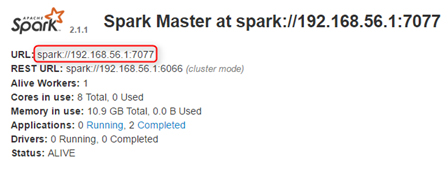
\includegraphics[width=1\linewidth]{spark-working}
	\caption{Spark Master - Adres URL węzła zarządzającego klastrem}
	\label{fig:stronaTytulowa}
\end{figure}

Kolejnym krokiem jest aktywacja wszystkich pozostałych maszyn jako węzły obliczeniowe. Wykonuje się to poprzez użycie komendy znajdującej się jak uprzednio w folderze \texttt{\hl{sbin}} katalogu głównego \textit{Apache Spark'a}: \\ \vspace{2mm}
\centerline{\texttt{\hl{start-slave.sh -c <max-cores> -m <max-memory ><master-url>}}, np.}
\centerline{\texttt{\hl{start-slave.sh -c 4 -m 2G spark://192.168.56.1:7077}}}
Jeśli wystąpią problemy z powyższą komendą, należy skorzystać z:\\
\centerline{\texttt{\hl{Spark-class org.apache.spark.deploy.worker.Worker }}}
\centerline{\texttt{\hl{-c <max-cores> -m <max-memory ><master-url>}}}
Jeśli węzły prawidłowo skomunikują się z głównym węzłem, będzie to widoczne
w panelu webowym głównej maszyny. \textbf{Klaster obliczeniowy został uruchomiony poprawnie}.
\pagebreak
\vspace*{1mm}
\section{Uruchomienie GRAVIsim}
Uruchamianie aplikacji należy rozpocząć od aktywowania właściwej wersji \textit{Python'a} (3.5)
najlepiej przy użyciu narzędzia \textit{Virtual-Env}. Dla tak przygotowanej konfiguracji
należy zainstalować wszystkie wymagane zależności \textit{Python'a} poprzez komendę:\vspace{2mm}
\centerline{\texttt{\hl{pip install -r requirements.txt}}}\vspace{2mm}
oraz wszystkie zależności aplikacji klienckiej poprzez komendę:\\\vspace{2mm}
\centerline{\texttt{\hl{bower install}}}\vspace{2mm}

Kolejnym krokiem jest uruchomienie klastra (instrukcja w poprzednim rozdziale) - bardzo ważne jest aby komendy
tworzenia klastra wywołane były w konfiguracji \textit{Python 3.5} (aktywnym wirtualnym
środowisku).
\\
\\
Aby zapewnić prawidłowe działanie \textit{logger’a} zaleca się zmianę ustawień logowania \textit{Sparka} poprzez zmianę poziomu logowania z \textit{\textbf{INFO}} na \textit{\textbf{WARN}}. W tym celu należy w pliku:\vspace{2mm}
 \centerline{\texttt{\hl{\%SPARK{\char`_}HOME/conf/log4j.properties}}}
\begin{framed}
Jeśli plik nie istnieje, należy powielić plik:\\ \vspace{2mm}
  \centerline{\texttt{\hl{\%SPARK{\char`_}HOME/conf/log4j.properties.template}}}

oraz zmienić jego nazwę na \texttt{\hl{log4j.properties}} 
\end{framed}
dokonać modyfikacji  następującego kodu: \\ \vspace{2mm}
  \centerline{\texttt{\hl{Log4j.rootCategory=INFO, console}, na}}
  \centerline{\texttt{\hl{Log4j.rootCategory=WARN, console}}}\vspace{2mm}

Następnie należy uruchomić wszystkie moduły:
\begin{enumerate}
\item Serwer: \texttt{\hl{python manage.py runserver}}
\item Sockets-Server: \texttt{\hl{python manage.py sockets-server}}
\item Spark-Scheduler: \texttt{\hl{python manage.py spark-scheduler <master-url>}}
\end{enumerate}

Komendy są blokujące w związku z czym zaleca się użycie kilku terminali lub uruchomieniu
komend w trybie odłączonym i przekierowaniu wyjścia do pliku zewnętrznego.\vspace{2mm}

Dodatkowo - na wszystkich maszynach oprócz maszyny głównej - należy podmontować folder
\texttt{\hl{media}} przy użyciu skryptu \texttt{\hl{mount.sh}} dostarczonym z aplikacją lub ręcznie przy użyciu
komendy \texttt{\hl{sshfs}}.\\
\vspace{2mm} Aplikacja dostępna jest pod adresem hosta głównego na porcie \textbf{\textit{8000}}, np.\\
\centerline{\texttt{\hl{http://localhost:8000}}}
\chapter{Instrukcja użytkownika}


\chapter{Badanie złożoności obliczeniowej}
\emph{Badania przeprowadzono w politechnicznym laboratorium komputerowym z wykorzystaniem 9 identycznych komputerów, z których jeden służył za główny serwer aplikacji oraz zarządcę klastra, a pozostałe 8 za węzły obliczeniowe (równolegle od 1 do 8 - zależnie od specyfikacji testu).}

\section{Zestaw konfiguracyjny}

Testy przeprowadzono dla wybranych zestawów konfiguracyjnych, gdzie parametrami były:
\begin{itemize}
\item Ilość węzłów obliczeniowych
\item Wielkość pliku wejściowego (ilość punktów masy)
\item Ilość iteracji symulacji
\end{itemize}
Każdy z węzłów obliczeniowych otrzymywał na wyłączność badań:
\begin{itemize}
\item 2 rdzenie (procesor i7 3.4MHz)
\item 2.0 GB pamięci RAM (DDR3)
\end{itemize}
W trakcie badania parametry oraz zasoby poszczególnych węzłów nie były zmieniane.\\
Symulacja ma charakter liniowy (liniowa charakterystyka iteracji) dlatego dla większych wartości istnieje możliwość dokładnej estymacji czasu obliczania w oparciu o empiryczne wyniki pomiarów dla wartości mniejszych.

\begin{figure}[h!]
	\centering
	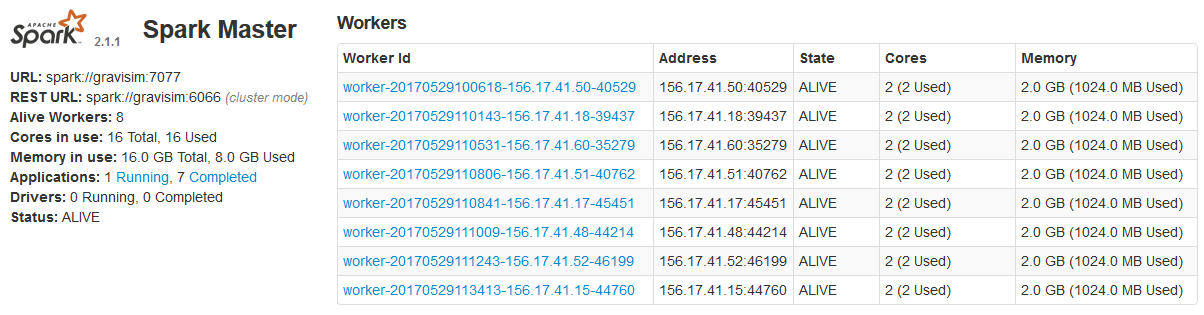
\includegraphics[width=1\linewidth]{klaster}
	\caption{Konfiguracja klastra wykorzystywanego do wykonywania pomiarów}
	\label{fig:stronaTytulowa}
\end{figure}

\pagebreak
\vspace*{1mm}
\section{Wyniki badań}
Wyniki badań oraz analizy przedstawia poniższe zestawienie tabelaryczne oraz wykresy.



\newcolumntype{P}[1]{>{\centering\arraybackslash}p{#1}}
\newcolumntype{M}[1]{>{\centering\arraybackslash}m{#1}}


\begin{table}[h]
  \centering
  \begin{tabular}{|c|c|c|c|c|c|c|}
    \hline
\textbf{Id} & \textbf{Węzły} & \textbf{CPU} & \textbf{RAM [GB]} & \textbf{Ilość punktów} & \textbf{Ilość iteracji} & \textbf{Wynik [s]} \\ 
\noalign{\hrule height 2pt }
1 & 1 & 2 & 2.0 & 100 & 500 & 215.67 \\ \hline
2 & 1 & 2 & 2.0 & 100 & 1000 & 421.42 \\ \hline
3 & 1 & 2 & 2.0 & 100 & 2000 & 821.24 \\ \hline
4 & 2 & 4 & 4.0 & 5000 & 10 & 256.46 \\ \hline
5 & 2 & 4 & 4.0 & 5000 & 20 & 528.44 \\ \hline
6 & 4 & 8 & 8.0 & 5000 & 10 & 94.43 \\ \hline
7 & 4 & 8 & 8.0 & 5000 & 20 & 201.78 \\ \hline
8 & 8 & 16 & 16.0 & 100 & 200 & 121.90 \\ \hline
9 & 8 & 16 & 16.0 & 100 & 500 & 238.60 \\ \hline
10 & 8 & 16 & 16.0 & 100 & 1000 & 537.77 \\ \hline
11 & 8 & 16 & 16.0 & 5000 & 10 & 58.99 \\ \hline
12 & 8 & 16 & 16.0 & 5000 & 20 & 116.29 \\ \hline
13 & 8 & 16 & 16.0 & 5000 & 500 & 2704.34 \\ \hline
  \end{tabular}
  \caption{Wyniki czasowe pomiarów wydajności klastra obliczeniowego}\label{tab1}
\end{table}
\begin{figure}[h!]
	\centering
	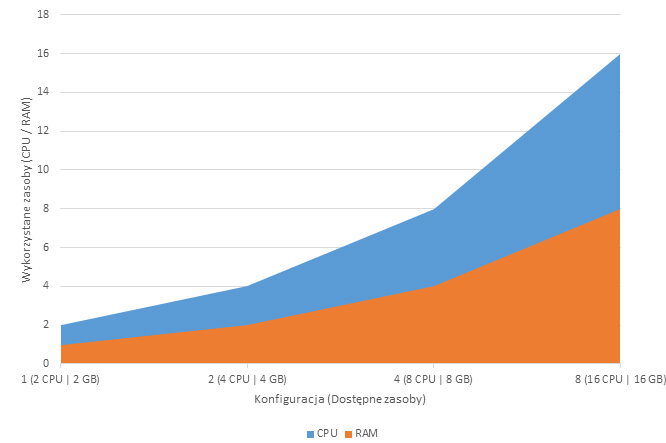
\includegraphics[width=0.93\linewidth]{wykres-4}
	\caption{Zużycie zasobów dla różnej konfiguracji klastra}
	\label{fig:stronaTytulowa}
\end{figure}
\begin{figure}[h!]
	\centering
	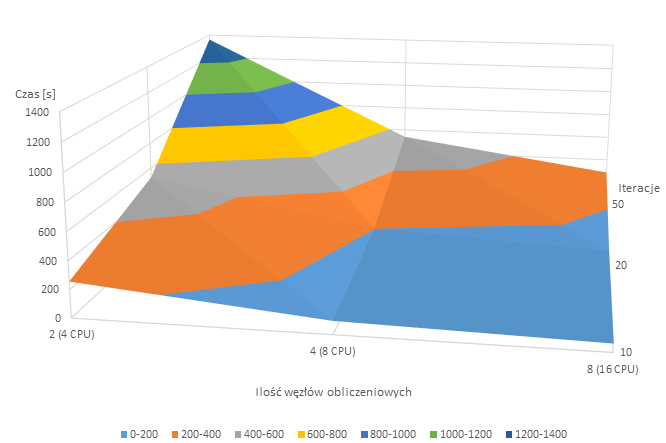
\includegraphics[width=1\linewidth]{wykres-1}
	\caption{Złożoność czasowa dla symulacji wielu punktów zależnie od ilości węzłów oraz ilości iteracji}
	\label{fig:stronaTytulowa}
\end{figure}

\begin{figure}[h!]
	\centering
	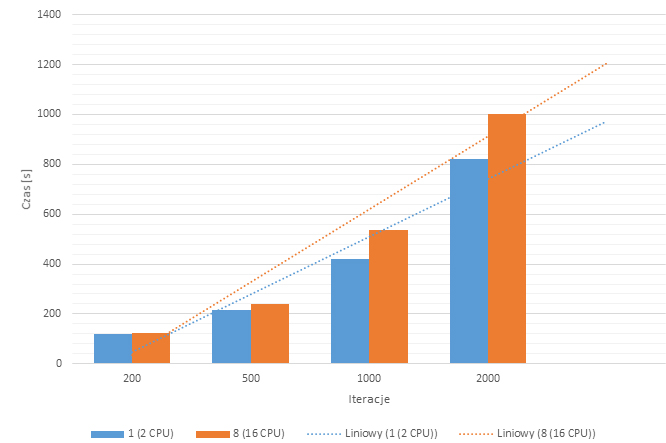
\includegraphics[width=1\linewidth]{wykres-2}
	\caption{Porównanie złożoności czasowych symulacji małej ilości punktów dla skrajnych konfiguracji klastra}
	\label{fig:stronaTytulowa}
\end{figure}


\begin{figure}[h!]
	\centering
	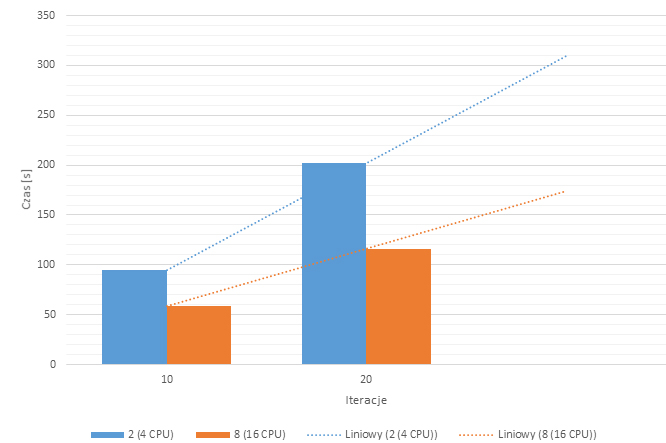
\includegraphics[width=1\linewidth]{wykres-3}
	\caption{Porównanie złożoności czasowych symulacji dużej ilości punktów dla skrajnych konfiguracji klastra}
	\label{fig:stronaTytulowa}
\end{figure}

\vspace*{1mm}
\section{Analiza wyników}
Na podstawie wyników przeprowadzonych badań można zaobserwować, iż wszystkie 3 badane parametry mają znaczący wpływ na czas wykonywania zadania.
Klaster obliczeniowy opiera się na komunikacji poszczególnych węzłów, która odbywając się poprzez sieć skutkuje znaczącym opóźnieniem w wykonywaniu zadania. Ma to ogromny wpływ dla zadań liczonych stosunkowo szybko (mała ilość punktów masy w symulacji), stąd też zaobserwowano, iż klaster o większej ilości węzłów obliczył to samo zadanie w czasie o 10-15\% dłuższym niż klaster składający się z 1 węzła. Dla większych zadań, narzut komunikacyjny staje się znikomo mały i czas tego samego zadania zależy tylko od dostępności zasobów.

\chapter{Podsumowanie i wnioski}

\mbox{}\pdfbookmark[0]{Spis rysunków}{spisRysunkow.1}
%\addcontentsline{toc}{chapter}{Spis rysunków}
\listoffigures*

\begin{flushleft}

\end{flushleft}
%{%
%\let\oldnumberline\numberline%
%\renewcommand{\numberline}{\figurename~\oldnumberline}%
%\listoffigures%
%}





%\bibliographystyle{plalpha}
\bibliographystyle{plabbrv}

%UWAGA: bibliotekę referencji należy przygotować samemu. Dobrym do tego narzędziem jest JabRef.
%       Nazwę przygotowanej biblioteki wpisuje się poniżej bez rozszerzenia 
%       (w tym przypadku jest to "dokumentacja.bib")


\chapterstyle{noNumbered}
\phantomsection % sets an anchor
\addcontentsline{toc}{chapter}{Indeks rzeczowy}
\printindex

\end{document}
